\chapter{Analisi degli eventi}
\section{Rally a Indianola, Iowa (14 gennaio 2024)}

Il 14 gennaio 2024 a Indianola, presso il Simpson College in Iowa, si è tenuto un importante rally elettorale di Donald Trump in vista dei caucus repubblicani.
Trump ha parlato ai suoi sostenitori, promettendo misure ancora più dure rispetto al passato, tra cui un forte rilancio della produzione di petrolio, deportazioni di immigrati irregolari e una politica estera improntata a rapporti diretti con leader come Putin e Kim Jong-un.
L’evento si è svolto in un clima molto freddo, ma ha visto una grande partecipazione di pubblico, sottolineando l’importanza dell’Iowa come primo stato a votare nelle primarie USA 2024.
Il rally ha avuto anche lo scopo di motivare i sostenitori a partecipare attivamente ai caucus del giorno successivo, fondamentali per la corsa alla nomination repubblicana. \\

\begin{figure}[H]
    \centering
    \begin{subfigure}[t]{0.48\textwidth}
        \centering
        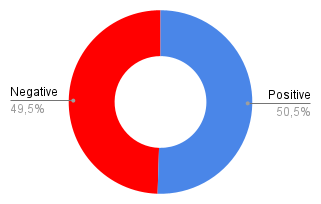
\includegraphics[width=\linewidth]{Immagini//Articolo1/Articolo 1 - Rapporto Totale Parole.png}
        \caption{Distribuzione del sentiment nelle parole analizzate.}
        \label{fig:totale-parole-a1}
    \end{subfigure}
    \hfill
    \begin{subfigure}[t]{0.48\textwidth}
        \centering
        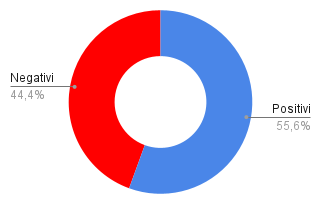
\includegraphics[width=\linewidth]{Immagini//Articolo1/Articolo 1 - Rapporto Totale Articoli.png}
        \caption{Distribuzione degli articoli per orientamento politico.}
        \label{fig:totale-articoli-a1}
    \end{subfigure}
    \caption{Articolo 1 - Analisi complessiva del corpus: parole e articoli.}
    \label{fig:analisi-totale-a1}

    \centering
    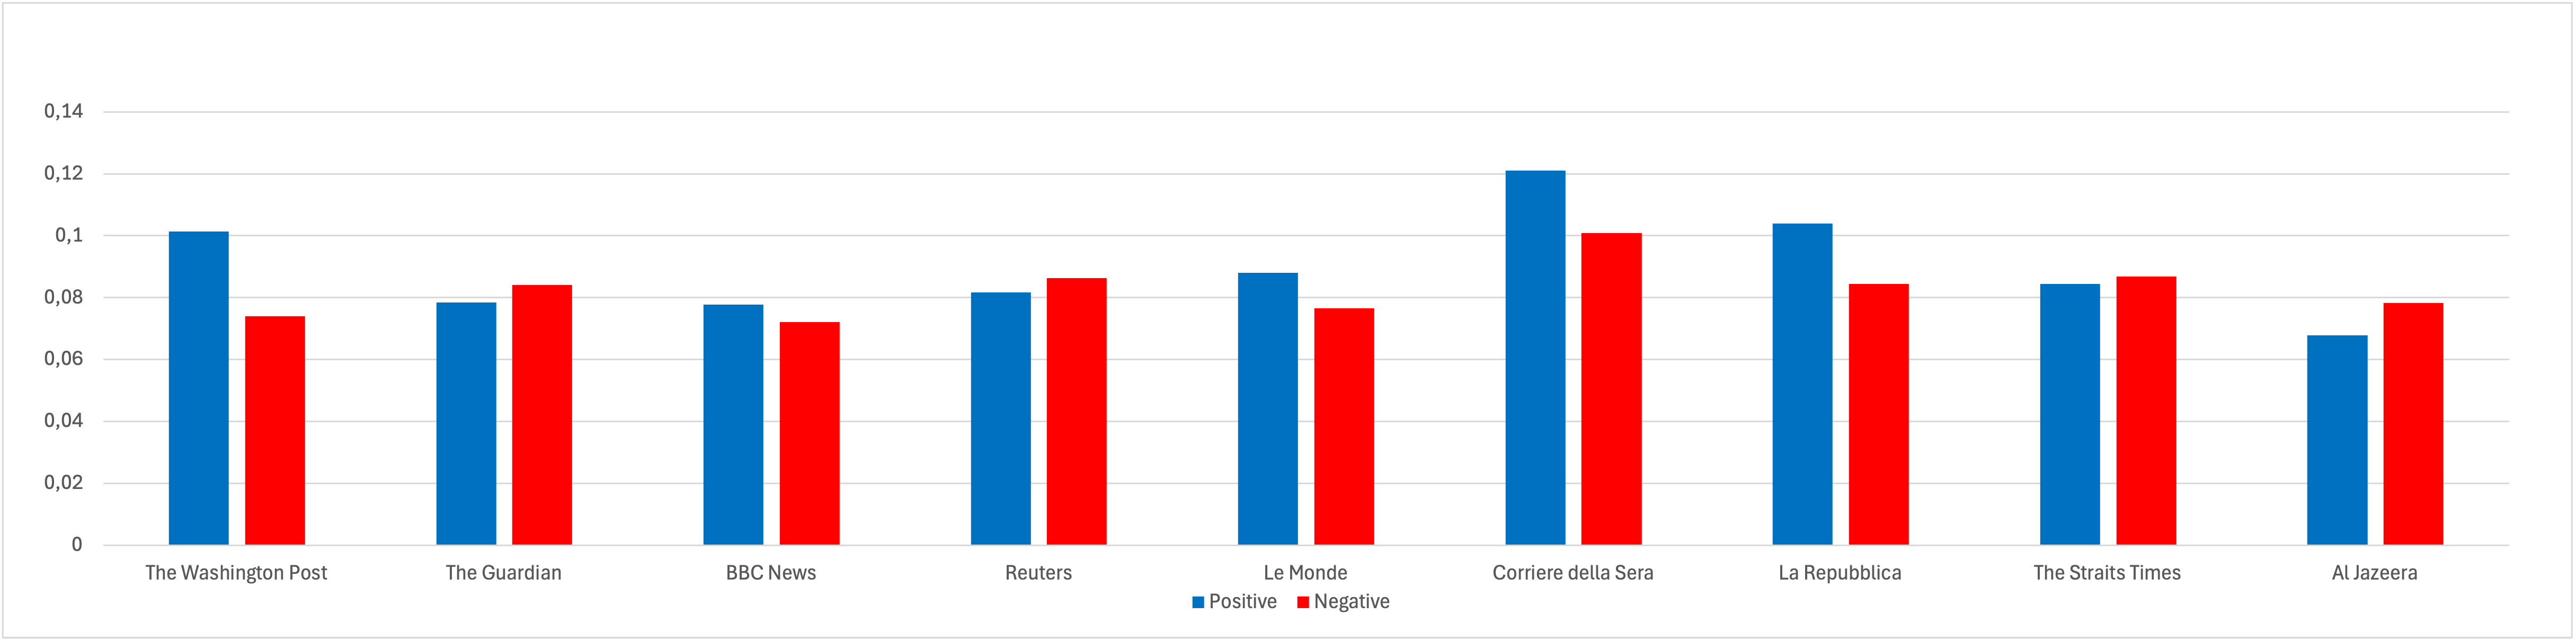
\includegraphics[width=1\linewidth]{Immagini//Articolo1/Articolo 1 - Analisi Grafica Risultati Totali.png}
    \caption{Articolo 1 - Distribuzione del sentiment negli articoli analizzati: confronto tra parole positive e negative.}
    \label{fig:risultati-totali-a1}
\end{figure}

I risultati illustrati evidenziano una distribuzione lessicale sostanzialmente bilanciata tra termini a connotazione positiva (\SI{50.5}{\percent}) e negativa (\SI{49.5}{\percent}) come evidenziato nella Figura~\ref{fig:totale-parole-a1}. Tale equilibrio linguistico suggerisce una narrazione mediatica complessivamente neutra dal punto di vista puramente semantico. Tuttavia, nonostante questa apparente neutralità, l'analisi del tono generale degli articoli (Figura~\ref{fig:totale-articoli-a1}) mostra che 5 articoli su 9, il \SI{55.6}{\percent}, assumono un'impostazione prevalentemente positiva, mentre 4 articoli su 9, il \SI{44.4}{\percent}, si caratterizza con un orientamento negativo.
Questa discrepanza tra il bilanciamento lessicale e la valutazione del tono complessivo (visualizzata graficamente nella Figura~\ref{fig:analisi-totale-a1}) può essere ricondotta a diversi fattori, tra cui il peso semantico attribuito alle parole chiave all'interno del contesto testuale, nonché la presenza di giudizi ambivalenti o contrastanti all'interno dei singoli articoli.
Per quanto riguarda l'orientamento politico delle fonti esaminate, la distribuzione risulta relativamente omogenea: si rilevano infatti quattro articoli provenienti da testate neutrali, tre da fonti con orientamento progressista e due da fonti di matrice conservatrice. Tale composizione suggerisce una copertura mediatica equilibrata, seppur con una lieve inclinazione critica.

\newpage
\section{Discorso al CPAC (24 febbraio 2024)}

Al CPAC 2024, tenutosi il 24 febbraio al National Harbor (Maryland), Donald Trump ha tenuto un discorso molto atteso davanti ai principali esponenti del movimento conservatore americano.
Nel suo intervento, Trump si è definito un “dissidente politico” e ha presentato le elezioni del 5 novembre come una sorta di “giorno della liberazione” per gli Stati Uniti.
Ha attaccato duramente l’amministrazione Biden, promesso di “salvare l’America” e ha ribadito i suoi temi chiave: lotta all’immigrazione irregolare, difesa dei valori tradizionali, revisione delle politiche economiche e dure critiche contro l’establishment di Washington.
Il discorso ha galvanizzato la platea, confermando il ruolo centrale di Trump nel partito repubblicano e tra i conservatori americani. \\

\begin{figure}[H]
    \centering
    \begin{subfigure}[t]{0.48\textwidth}
        \centering
        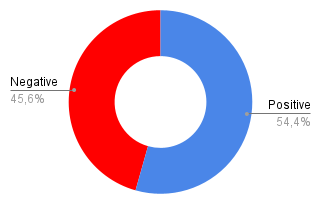
\includegraphics[width=\linewidth]{Immagini//Articolo2/Articolo 2 - Rapporto Totale Parole.png}
        \caption{Distribuzione del sentiment nelle parole analizzate.}
        \label{fig:totale-parole-a2}
    \end{subfigure}
    \hfill
    \begin{subfigure}[t]{0.48\textwidth}
        \centering
        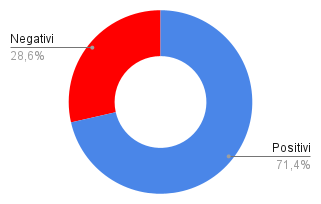
\includegraphics[width=\linewidth]{Immagini//Articolo2/Articolo 2 - Rapporto Totale Articoli.png}
        \caption{Distribuzione degli articoli per orientamento politico.}
        \label{fig:totale-articoli-a2}
    \end{subfigure}
    \caption{Articolo 2 - Analisi complessiva del corpus: parole e articoli.}
    \label{fig:analisi-totale-a2}

    \centering
    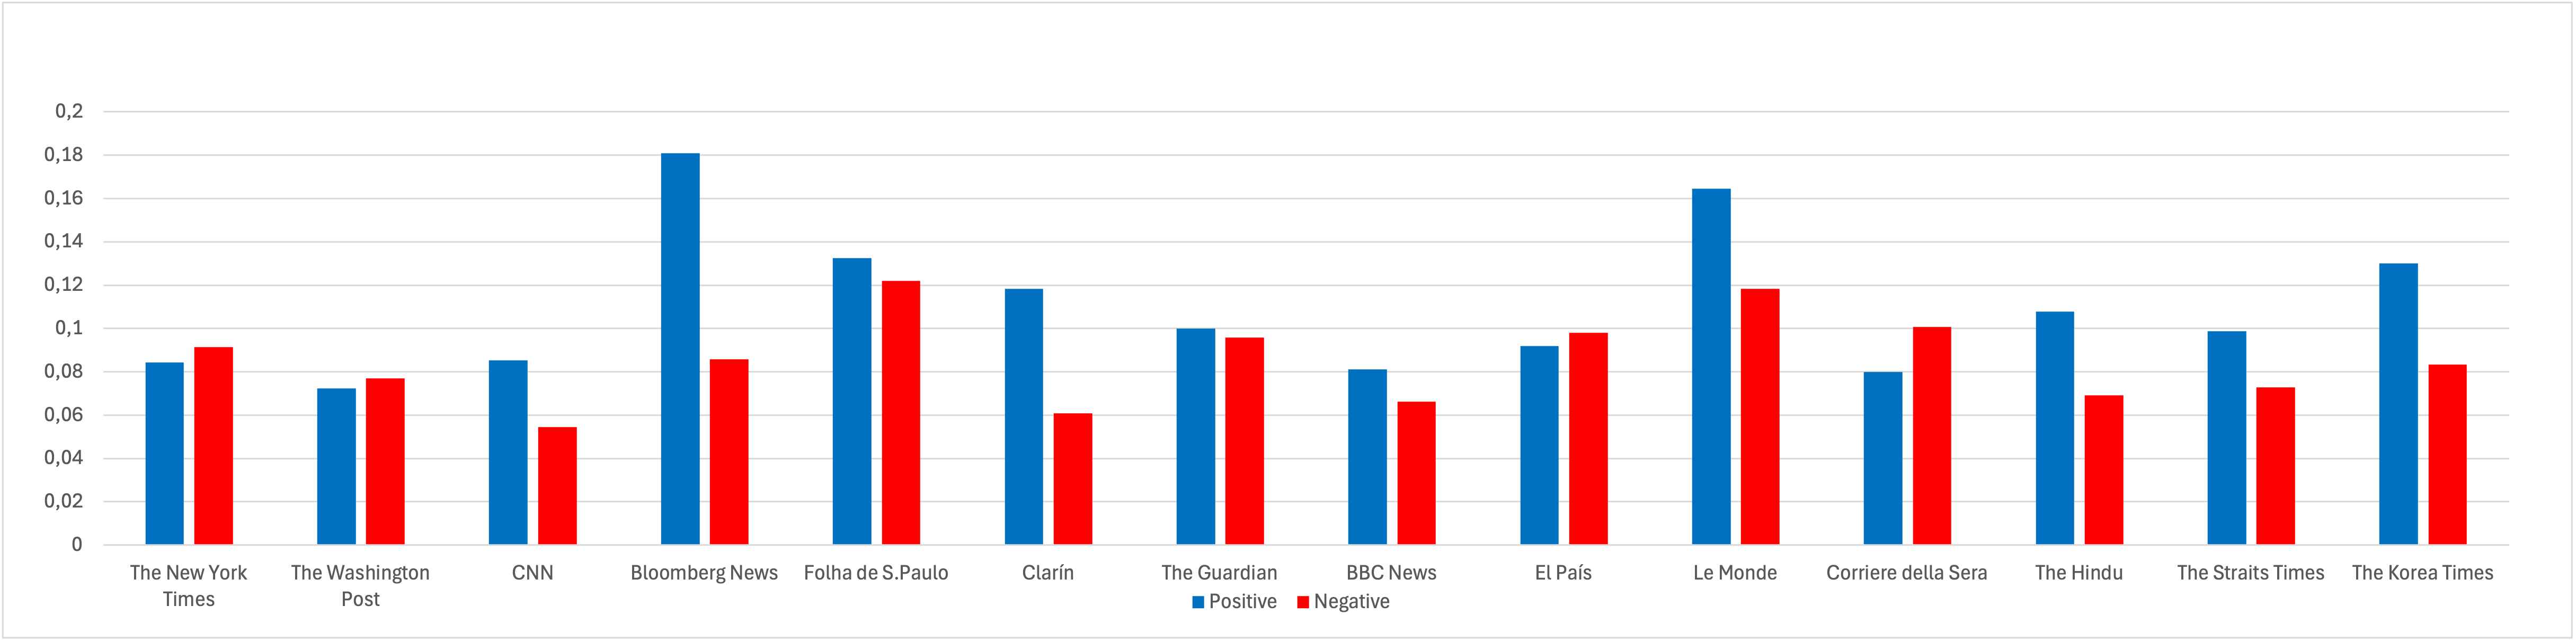
\includegraphics[width=1\linewidth]{Immagini//Articolo2/Articolo 2 - Analisi Grafica Risultati Totali.png}
    \caption{Articolo 2 - Distribuzione del sentiment negli articoli analizzati: confronto tra parole positive e negative.}
    \label{fig:risultati-totali-a2}
\end{figure}

In questo caso vi è una prevalenza di articoli provenienti da testate progressiste (6), rispetto a quelli riconducibili a fonti conservatrici (5) e neutrali (3). Tale distribuzione suggerisce una copertura mediatica leggermente orientata verso una prospettiva progressista, che potrebbe influenzare il tono complessivo della narrazione.
L'analisi del sentiment lessicale (Figura~\ref{fig:totale-parole-a2}) mostra una predominanza di termini a connotazione positiva (\SI{54.4}{\percent}) rispetto a quelli negativi (\SI{45.6}{\percent}), questo si riflette anche nel tono generale degli articoli (Figura~\ref{fig:totale-articoli-a2}), dove la maggioranza (10 articoli su 14, pari al \SI{71.4}{\percent}) è stata classificata come positiva, mentre solo 4 articoli (\SI{28.6}{\percent}) risultano avere un tono negativo.
Dal punto di vista delle parole utilizzate, il rapporto tra termini positivi e negativi suggerisce una narrazione favorevole, in linea con la classificazione degli articoli. Da notare che anche testate generalmente considerate neutrali o conservatrici hanno espresso, in vari casi, un tono positivo.
In conclusione, la copertura mediatica del discorso al CPAC 2024 appare complessivamente positiva, sia in termini quantitativi (numero di articoli con tono favorevole) sia qualitativi (prevalenza di lessico positivo), nonostante la leggera prevalenza di fonti progressiste. Ciò suggerisce una ricezione generalmente benevola del contenuto del discorso, indipendentemente dall’orientamento politico delle testate analizzate.

\newpage
\section{Nomination repubblicana (18 luglio 2024)}
Il 18 luglio 2024, a Milwaukee, Donald Trump ha accettato la nomination repubblicana alla presidenza, pochi giorni dopo un attentato in cui è rimasto ferito. Con una benda sull'orecchio, ha promesso di "salvare l'America", unire il paese e ripristinare il "sogno americano". 
Pur aprendo con toni più concilianti, ha poi attaccato i democratici e ribadito le sue promesse classiche: chiusura delle frontiere, deportazioni, rilancio del petrolio e tagli alle tasse.
Il discorso si è concluso in un clima di entusiasmo con una pioggia di palloncini. \\

\begin{figure}[H]
    \centering
    \begin{subfigure}[t]{0.48\textwidth}
        \centering
        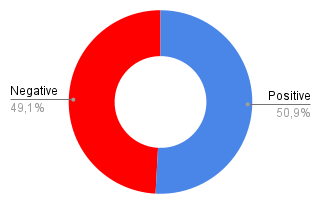
\includegraphics[width=\linewidth]{Immagini//Articolo3/Articolo 3 - Rapporto Totale Parole.png}
        \caption{Distribuzione del sentiment nelle parole analizzate.}
        \label{fig:totale-parole-a3}
    \end{subfigure}
    \hfill
    \begin{subfigure}[t]{0.48\textwidth}
        \centering
        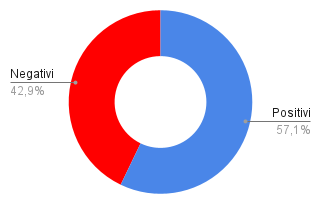
\includegraphics[width=\linewidth]{Immagini//Articolo3/Articolo 3 - Rapporto Totale Articoli.png}
        \caption{Distribuzione degli articoli per orientamento politico.}
        \label{fig:totale-articoli-a3}
    \end{subfigure}
    \caption{Articolo 3 - Analisi complessiva del corpus: parole e articoli.}
    \label{fig:analisi-totale-a3}

    \centering
    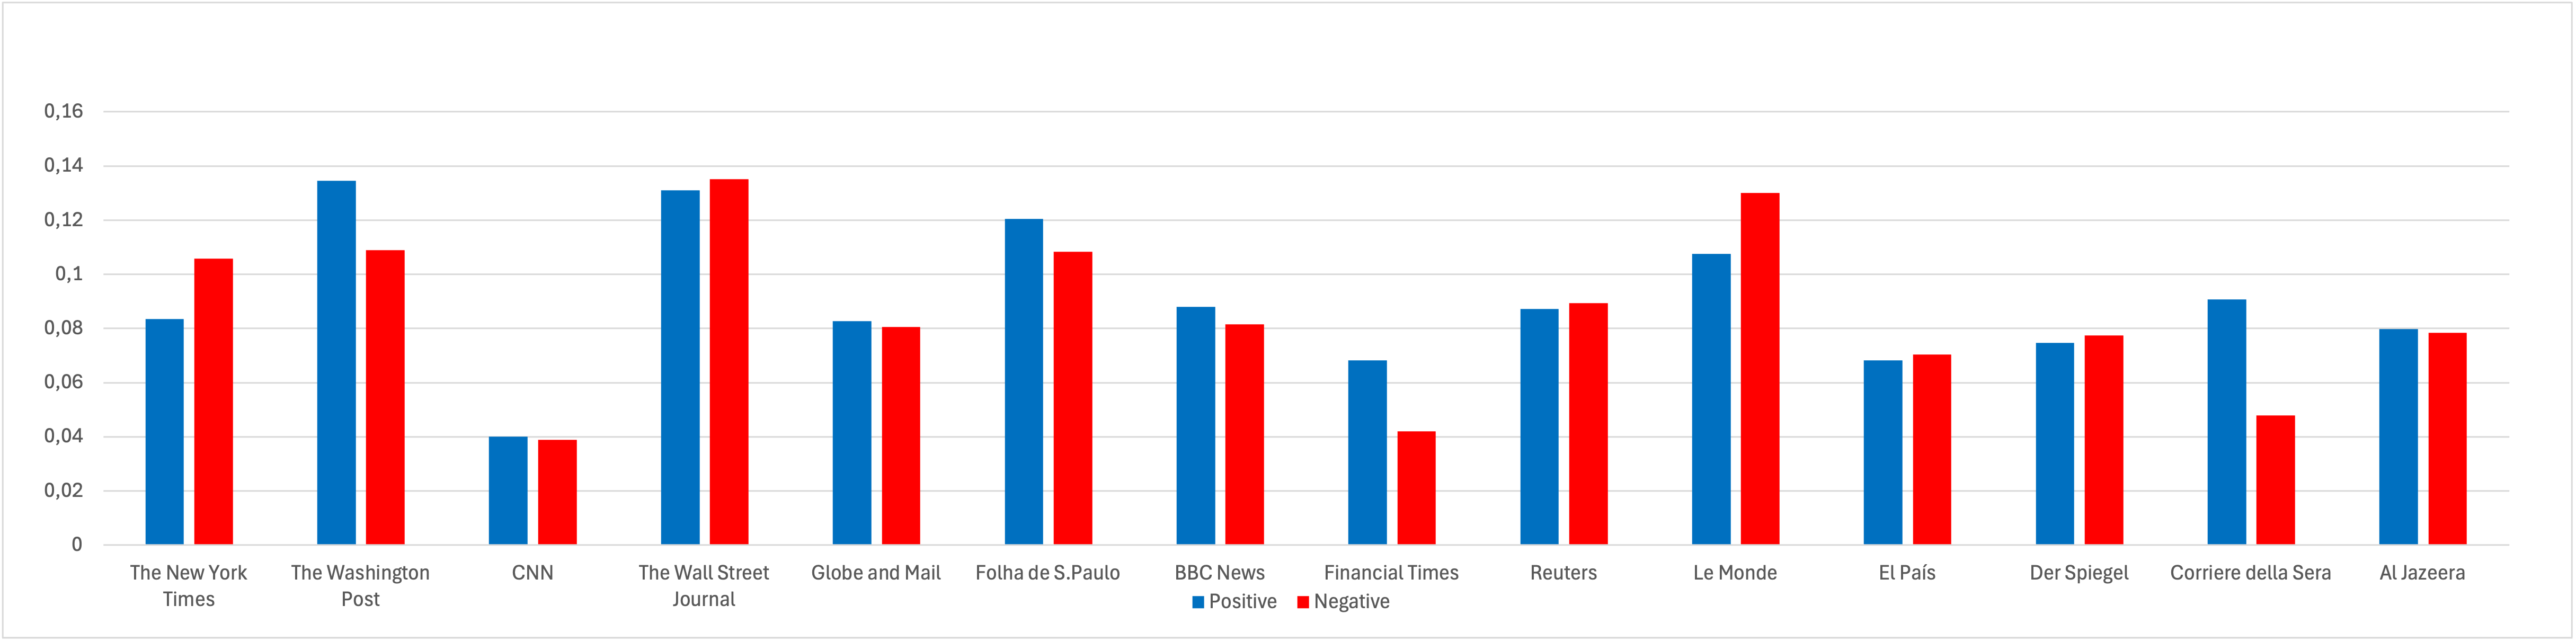
\includegraphics[width=1\linewidth]{Immagini//Articolo3/Articolo 3 - Analisi Grafica Risultati Totali.png}
    \caption{Articolo 3 - Distribuzione del sentiment negli articoli analizzati: confronto tra parole positive e negative.}
    \label{fig:risultati-totali-a3}
\end{figure}
In questo caso vi è una netta predominanza di articoli progressisti (8) rispetto a quelli neutrali (4) e conservatori (2), indicando una copertura mediatica fortemente polarizzata. Nonostante questa asimmetria politica, l'analisi lessicale (Figura~\ref{fig:totale-parole-a3}) rivela un sostanziale equilibrio tra termini positivi (\SI{50.9}{\percent}) e negativi (\SI{49.1}{\percent}), suggerendo che il linguaggio utilizzato mantiene un'apparente neutralità semantica. Tuttavia, il tono complessivo degli articoli (Figura~\ref{fig:totale-articoli-a3}) presenta una lieve differenza: 8 articoli su 14, il \SI{57.1}{\percent}, sono stati classificati come positivi contro i 6 su 14, \SI{42.9}{\percent}, negativi. Questa divergenza potrebbe derivare dall'enfasi posta dai media progressisti sugli aspetti drammatici dell'attentato subito da Trump (citato come elemento negativo in contesti positivi) o dalla tendenza dei conservatori a celebrare il "miracoloso salvataggio" come simbolo di resilienza, dimostrando come eventi traumatici possano generare narrazioni complesse dove elementi critici e positivi si intrecciano in modo controintuitivo.

\newpage
\section{Discorso di vittoria (6 novembre 2024)}

La notte del 6 novembre 2024, a West Palm Beach, Donald Trump ha tenuto il suo discorso di vittoria dopo le elezioni presidenziali.
Ha parlato di “età dell’oro per l’America”, promettendo di mantenere le sue promesse, unire il Paese e “fermare le guerre”.
Ha ringraziato la famiglia, i sostenitori e ha definito la sua vittoria “il più grande comeback della storia”, sottolineando il mandato ricevuto dagli americani e la conquista di diversi stati chiave.
Ha elogiato Elon Musk e ha promesso che l’America tornerà grande. \\

\begin{figure}[H]
    \centering
    \begin{subfigure}[t]{0.48\textwidth}
        \centering
        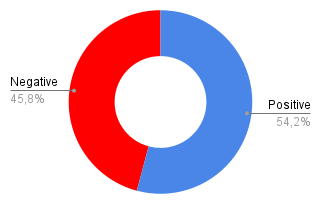
\includegraphics[width=\linewidth]{Immagini//Articolo4/Articolo 4 - Rapporto Totale Parole.png}
        \caption{Distribuzione del sentiment nelle parole analizzate.}
        \label{fig:totale-parole-a4}
    \end{subfigure}
    \hfill
    \begin{subfigure}[t]{0.48\textwidth}
        \centering
        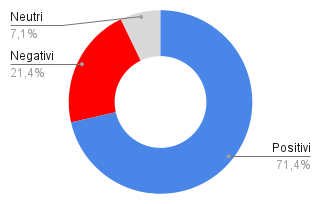
\includegraphics[width=\linewidth]{Immagini//Articolo4/Articolo 4 - Rapporto Totale Articoli.png}
        \caption{Distribuzione degli articoli per orientamento politico.}
        \label{fig:totale-articoli-a4}
    \end{subfigure}
    \caption{Articolo 4 - Analisi complessiva del corpus: parole e articoli.}
    \label{fig:analisi-totale-a4}

    \centering
    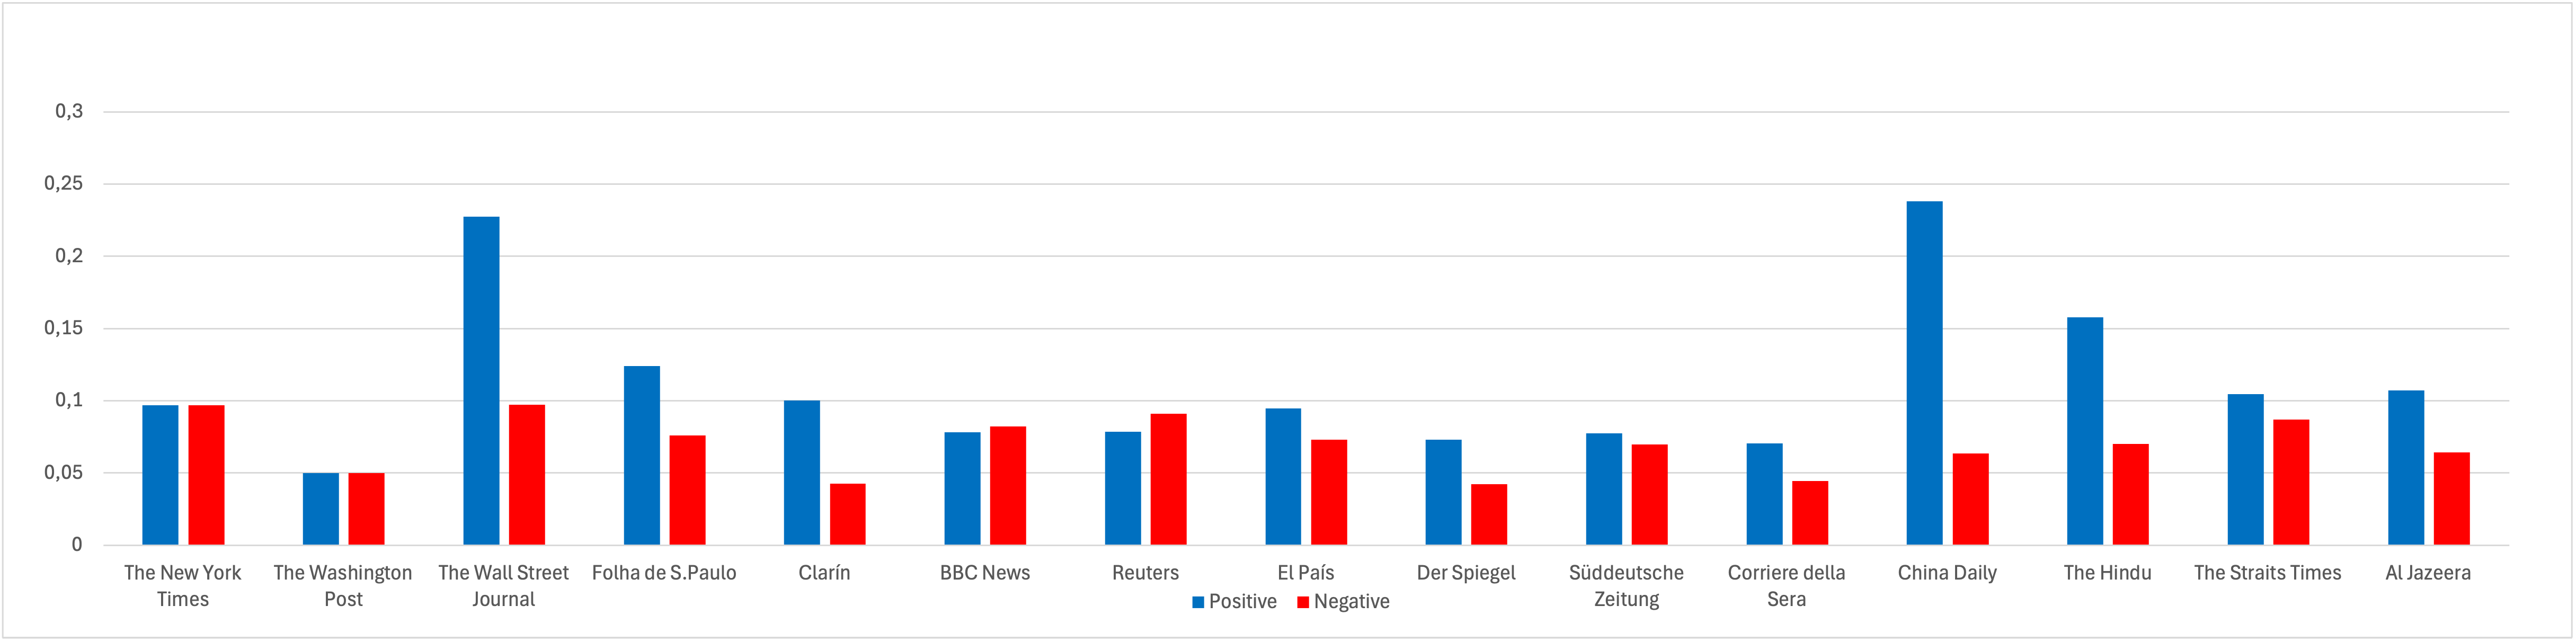
\includegraphics[width=1\linewidth]{Immagini//Articolo4/Articolo 4 - Analisi Grafica Risultati Totali.png}
    \caption{Articolo 4 - Distribuzione del sentiment negli articoli analizzati: confronto tra parole positive e negative.}
    \label{fig:risultati-totali-a4}
\end{figure}
L'analisi del discorso di vittoria elettorale rivela una marcata polarizzazione nel tono degli articoli, con una schiacciante maggioranza di contenuti positivi, 10 articoli su 14 (\SI{71.8}{\percent}), rispetto a quelli negativi, 3 articoli su 14 (\SI{21.4}{\percent}), e neutrali, 1 articolo su 14 (\SI{7}{\percent}) (Figura~\ref{fig:totale-articoli-a4}). Questo quadro contrasta parzialmente con l'analisi lessicale (Figura~\ref{fig:totale-parole-a4}), che mostra un equilibrio più moderato tra termini positivi (\SI{54.2}{\percent}) e negativi (\SI{45.8}{\percent}). La discrepanza evidenzia come elementi contestuali - come il clima di celebrazione post-elettorale e le immagini simboliche della vittoria - abbiano influenzato il tono complessivo oltre la mera frequenza di parole polarizzate. Particolarmente significativo è il minimo apporto di articoli neutrali (1 articolo su 14, il \SI{7}{\percent}), che suggerisce come l'evento abbia spinto i media a prendere posizione netta, sia in senso celebrativo (specialmente tra i conservatori) sia critico (tra i progressisti). L'uso strategico di espressioni come "età dell'oro" da parte di Trump par aver funzionato come frame dominante, mentre le critiche sono state relegate a un ruolo minoritario nonostante costituissero quasi la metà del lessico utilizzato.

\newpage
\section{Discorso inaugurale (20 gennaio 2025)}

Il 20 gennaio 2025, Donald Trump ha tenuto il discorso di insediamento come 47º Presidente degli Stati Uniti a Washington.
Ha dichiarato che “l’Età dell’Oro dell’America inizia proprio ora”, promettendo di mettere “America al primo posto”, ripristinare la sovranità, la sicurezza e la giustizia, e porre fine all’uso politico del Dipartimento di Giustizia.
Ha annunciato una “rivoluzione del buon senso”, la dichiarazione di emergenza nazionale al confine sud, il ritorno della politica “Remain in Mexico”, la lotta ai cartelli della droga e il rilancio della produzione energetica nazionale.
Ha ringraziato le comunità nere e ispaniche per il sostegno, ha promesso unità nazionale e ha sottolineato che “il declino dell’America è finito”.
Ha concluso affermando che il suo obiettivo sarà essere “pacificatore e unificatore”, rilanciando il sogno americano e la fiducia nel futuro del Paese.

\begin{figure}[H]
    \centering
    \begin{subfigure}[t]{0.48\textwidth}
        \centering
        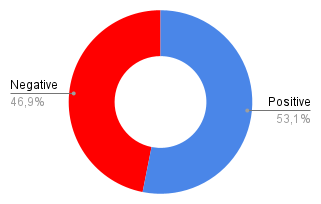
\includegraphics[width=\linewidth]{Immagini//Articolo5/Articolo 5 - Rapporto Totale Parole.png}
        \caption{Distribuzione del sentiment nelle parole analizzate.}
        \label{fig:totale-parole-a5}
    \end{subfigure}
    \hfill
    \begin{subfigure}[t]{0.48\textwidth}
        \centering
        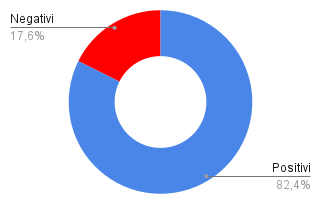
\includegraphics[width=\linewidth]{Immagini//Articolo5/Articolo 5 - Rapporto Totale Articoli.png}
        \caption{Distribuzione degli articoli per orientamento politico.}
        \label{fig:totale-articoli-a5}
    \end{subfigure}
    \caption{Articolo 5 - Analisi complessiva del corpus: parole e articoli.}
    \label{fig:analisi-totale-a5}

    \centering
    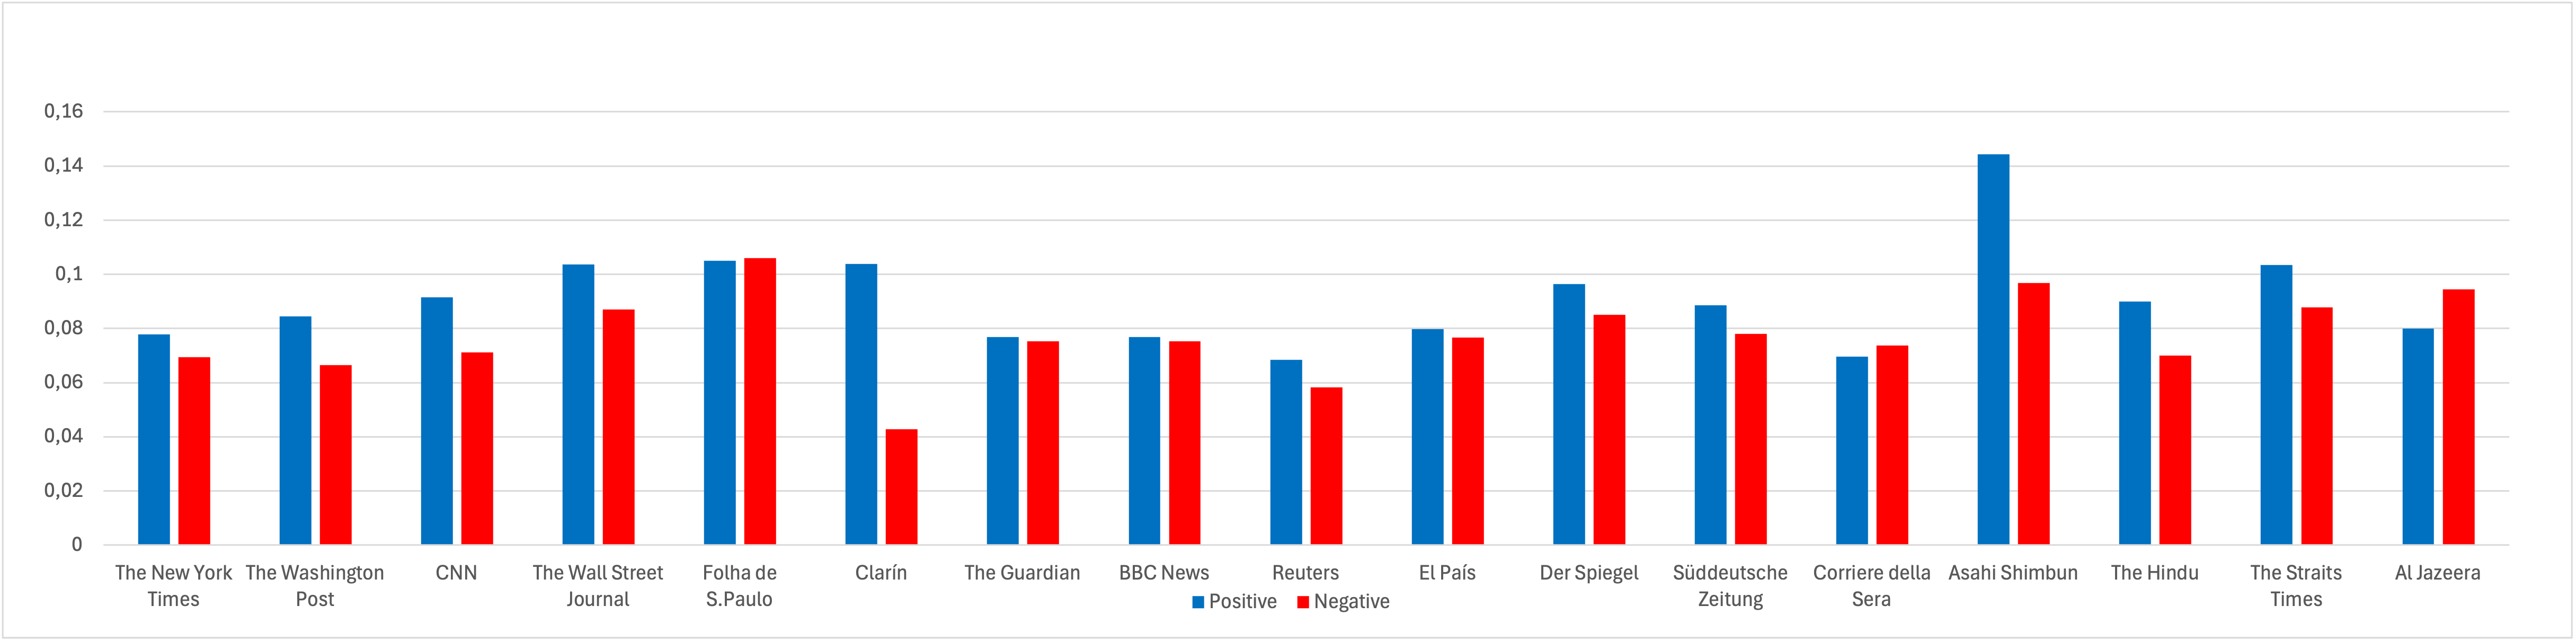
\includegraphics[width=1\linewidth]{Immagini//Articolo5/Articolo 5 - Analisi Grafica Risultati Totali.png}
    \caption{Articolo 5 - Distribuzione del sentiment negli articoli analizzati: confronto tra parole positive e negative.}
    \label{fig:risultati-totali-a5}
\end{figure}
L'analisi del discorso inaugurale mostra una predominanza di articoli progressisti (8 su 17) rispetto a quelli neutrali (5 su 17) e conservatori (4 su 17), indicando una copertura mediatica con significativa polarizzazione politica. Nonostante tale squilibrio, l'analisi lessicale (Figura~\ref{fig:totale-parole-a5}) rivela un lieve vantaggio dei termini positivi (\SI{53.1}{\percent}) rispetto a quelli negativi (\SI{46.9}{\percent}), riflettendo probabilmente il tono istituzionale ed unificante tipico di un discorso d'insediamento. Sorprendentemente, il \SI{82.4}{\percent} degli articoli è stato classificato come positivo nel tono complessivo, contro solo il \SI{17.6}{\percent} negativo (Figura~\ref{fig:totale-articoli-a6}). Questa marcata discrepanza tra la significativa presenza di lessico negativo e il tono prevalentemente positivo degli articoli può essere spiegata attraverso tre fattori chiave: 
\begin{enumerate}
    \item L'uso da parte dei media progressisti di citazioni dirette del discorso (positive) in contesti critici
    \item L'enfasi mediatica sugli aspetti rituali e simbolici della cerimonia presidenziale
    \item La tendenza dei conservatori a celebrare l'evento come ripristino della tradizione
\end{enumerate}
L'estrema rarità di articoli negativi (\SI{17.6}{\percent}) suggerisce che persino i media dell'opposizione abbiano riservato un trattamento rispettoso al momento istituzionale, pur mantenendo riserve sulle politiche annunciate.

\newpage
\section{Forum economico mondiale a Davos (23 gennaio 2025)}

A Davos, il 23 gennaio 2025, Trump ha promesso una "nuova età dell'oro" per gli USA, con l'obiettivo di renderli "più forti, ricchi e uniti".
Ha criticato le politiche economiche precedenti, promettendo tagli alle tasse, meno regolamentazioni e rilancio energetico.
Ha annunciato la fine del Green New Deal e dazi per chi produce all'estero.
Ha chiesto più spesa militare alla NATO, ha rivendicato meritocrazia e libertà di parola, e ha promesso di fermare l'immigrazione illegale.
Ha sottolineato investimenti record in America e auspicato la fine della guerra in Ucraina e un ruolo USA nei negoziati di pace in Medio Oriente. \\

\begin{figure}[H]
    \centering
    \begin{subfigure}[t]{0.48\textwidth}
        \centering
        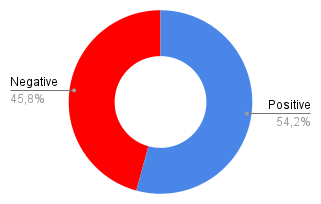
\includegraphics[width=\linewidth]{Immagini//Articolo6/Articolo 6 - Rapporto Totale Parole.png}
        \caption{Distribuzione del sentiment nelle parole analizzate.}
        \label{fig:totale-parole-a6}
    \end{subfigure}
    \hfill
    \begin{subfigure}[t]{0.48\textwidth}
        \centering
        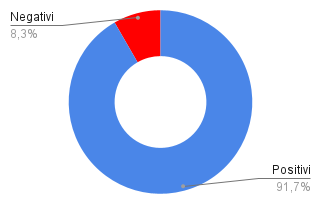
\includegraphics[width=\linewidth]{Immagini//Articolo6/Articolo 6 - Rapporto Totale Articoli.png}
        \caption{Distribuzione degli articoli per orientamento politico.}
        \label{fig:totale-articoli-a6}
    \end{subfigure}
    \caption{Articolo 6 - Analisi complessiva del corpus: parole e articoli.}
    \label{fig:analisi-totale-a6}

    \centering
    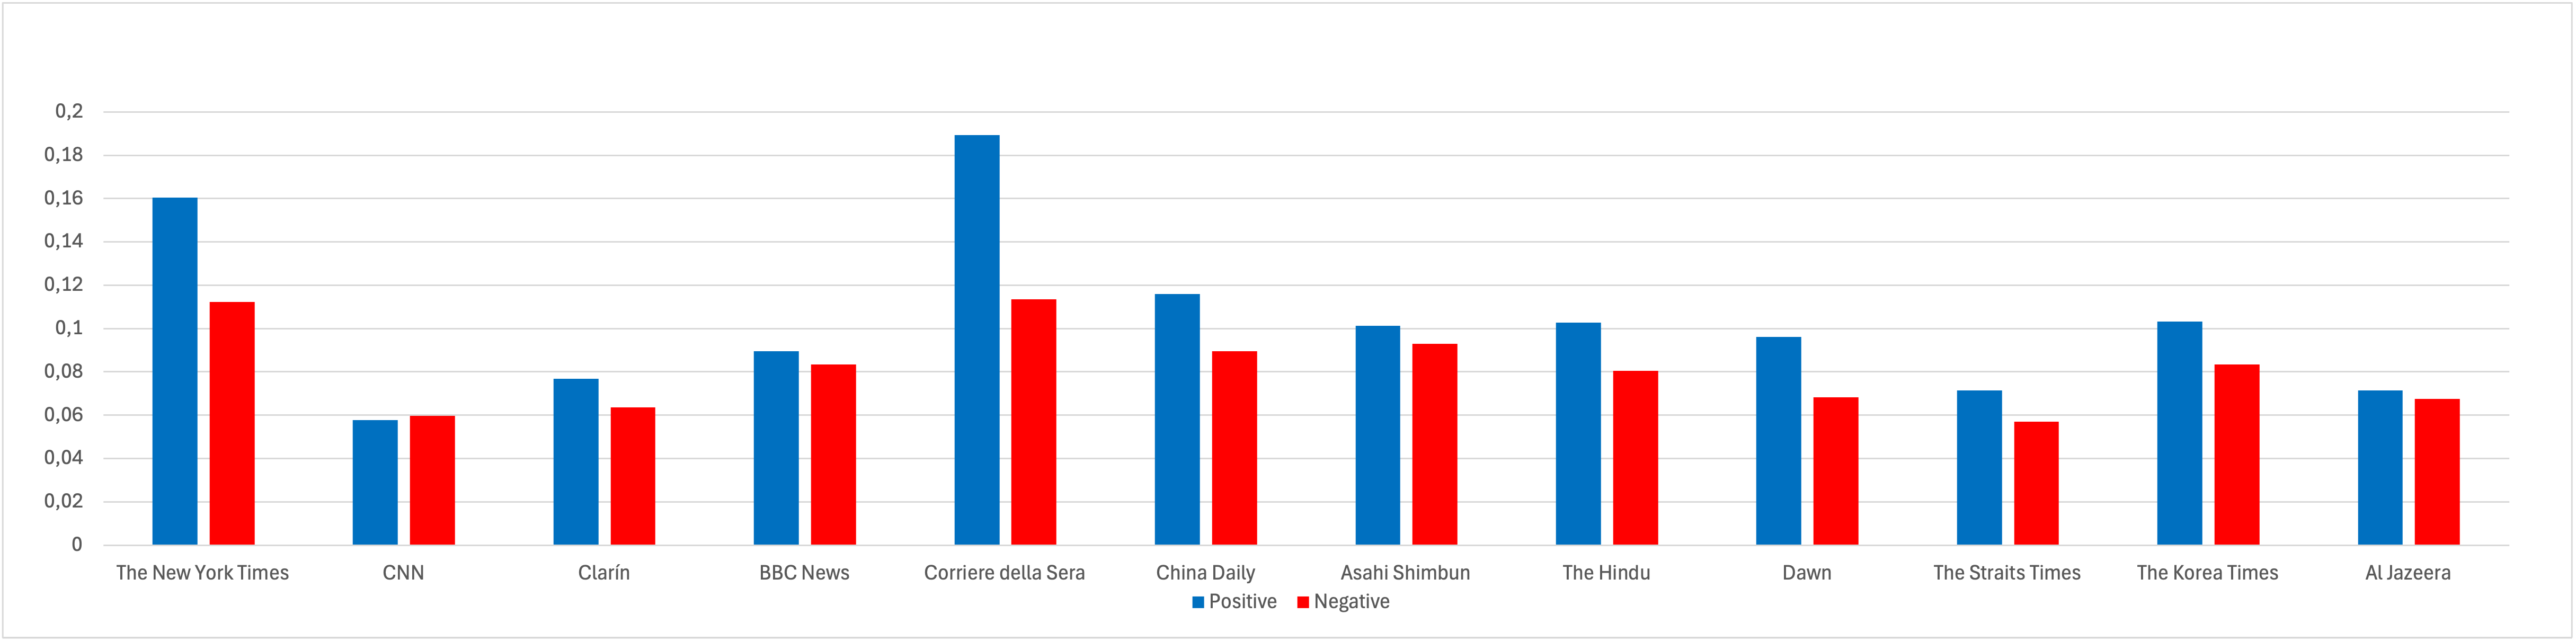
\includegraphics[width=1\linewidth]{Immagini//Articolo6/Articolo 6 - Analisi Grafica Risultati Totali.png}
    \caption{Articolo 6 - Distribuzione del sentiment negli articoli analizzati: confronto tra parole positive e negative.}
    \label{fig:risultati-totali-a6}
\end{figure}
L'analisi del discorso al World Economic Forum effettuata su una distribuzione equilibrata tra articoli progressisti, neutrali e conservatori (4 ciascuno), mostra un tono complessivo straordinariamente positivo: 11 articoli su 12, il \SI{91.7}{\percent}, sono stati classificati come favorevoli, contro solo 1 articolo su 12, l'\SI{8.3}{\percent}, critico  (Figura~\ref{fig:totale-articoli-a6}). Questo risultato contrasta parzialmente con l'analisi lessicale (Figura~\ref{fig:totale-parole-a6}), dove le parole positive (\SI{54.2}{\percent}) superano quelle negative (\SI{45.8}{\percent}) con un margine più contenuto. La marcata discrepanza tra il \SI{45.9}{\percent} di lessico negativo ed il singolo articolo critico suggerisce che: 
\begin{enumerate}
    \item I media abbiano generalmente "normalizzato" le controversie (dazi, abbandono del Green New Deal) inserendole in un frame complessivo di sviluppo economico
    \item Il contesto internazionale del WEF abbia indotto un trattamento più istituzionale
    \item La retorica trumpiana di "nuova età dell'oro" abbia funzionato da potente cornice interpretativa. 
\end{enumerate}
È particolarmente significativo come anche i media progressisti abbiano adottato prevalentemente un tono positivo, concentrando le critiche in specifici punti piuttosto che nell'interpretazione globale dell'evento.